\documentclass{deliverablereport}

\usepackage{pdfpages}
\usepackage{multirow}
\usepackage{doi}
\usepackage{hyperref}
\hypersetup{
  colorlinks=true,
  urlcolor=cyan,
  linkcolor=blue,
  citecolor=blue,
}

\deliverable{component-architecture}{hpc-configure}
\deliverydate{XX/YY/201Z}
\duedate{31/08/2019 (M48)}
\author{Alexis Breust, Jean-Guillaume Dumas, Clément Pernet, Hongguang Zhu}

\newcommand{\fflasffpack}{\textsc{fflas-ffpack}\xspace}
\begin{document}
\maketitle
% This will be the abstract, fetched from the github description
\githubissuedescription

% write the report here


%%%%%%%%%%%%%%%%%%%%%%%%%%%%%%%%%%%%%%%%%%%%%%%%%%%%%%%%%%%%%%
\section{Introduction}

%%%%%%%%%%%%%%%%%%%%%%%%%%%%%%%%%%%%%%%%%%%%%%%%%%%%%%%%%%%%%%
\section{Number Theory}

PARI-MT and the difficulty of composing a threaded systems into another.

%%%%%%%%%%%%%%%%%%%%%%%%%%%%%%%%%%%%%%%%%%%%%%%%%%%%%%%%%%%%%%
\section{Finite field linear algebra}

\subsection{Context}

Finite field linear algebra is a core building block in computational mathematics and deliver high computing throughput
to a wide range of applications, including number theory, group theory, combinatorics, etc. \SageMath relies on the
\fflasffpack library for its critical linear algebra operations on prime fields of less than 23 bits and consequently
also for numerous computations with multiprecision integer matrices.  

The \fflasffpack library had some preliminary support for multi-core parallelism for matrix
multiplication and Gaussian elimination.
Instead of being tight to a specific parallel language, the library uses a Domain Specific Language, Paladin~\cite{paladin},
to provide the library programmer with unique API for writing parallel code, which is then translated into 
OpenMP~\cite{openmp}, Cilk~\cite{cilk}, Intel-TBB~\cite{tbb}, or XKaapi~\cite{xkaapi} directives. Beside portability and independence from
a given technology, this also makes it possible to benchmark and compare how parallel runtime perform. This is
particularly important here, since many of the compute intensive routines of \fflasffpack share specificities that are
often challenges for parallel runtime:
\begin{description}
\item[Recursion] by design,  sub-cubic linear algebra algorithms are recursive and so are most routines in the
  library.
\item[Heterogeneity] many exact computations must deal with data with size unknown before their actual computation. For
  instance rank deficiencies in Gaussian elimination may generates a block decomposition of varying dimensions and
  therefore computing tasks will have heterogeneous load.
\item[Fine grain task parallelism] the combination of the two above constraints lead to consider recursive task
  parallelism with fine grain, so that a workstealing engine could efficiently balance the heterogeneity. However,
  recursive tasks have been for a long time rather inefficient in e.g. OpenMP implementations, and the ability to handle
  numerous fine grain tasks is also demanding on parallel runtimes.
\end{description}

\subsection{Integration within \SageMath}

The main tasks for the exposition of the parallel routines of \fflasffpack in \SageMath were the following:
\begin{enumerate}
\item improving existing parallel code for Gaussian elimination and matrix multiplication in the \fflasffpack library;
\item adding new parallel routines in \fflasffpack for the most commonly used operations in \SageMath: the determinant,
  the echelon form, the rank, and the solution of a linear system;
\item connecting these parallel routines in \SageMath  providing  the user
  with a precise control on the number of threads allocated to the linear algebra routines. 
\end{enumerate}

The first two items involved 15 pull-requests, merged and released in
\texttt{fflas-ffpack-2.4.3}\footnote{\url{https://github.com/linbox-team/fflas-ffpack/releases/tag/2.4.3}}. This release
was produced simultaneously with that of the two other libraries in the \Linbox
ecosystem: \texttt{givaro-4.1.1}\footnote{\url{https://github.com/linbox-team/givaro/releases/tag/4.1.1}} and
\texttt{linbox-1.6.3}\footnote{\url{https://github.com/linbox-team/linbox/releases/tag/v1.6.3}} then integrated into \SageMath
in tickets
\begin{itemize}
\item  \url{https://trac.sagemath.org/ticket/26932} and
\item  \url{https://trac.sagemath.org/ticket/27444},
\end{itemize}
which will appear in release 8.9 of \SageMath.

As a side note, the integration of these new releases including the contributions to \delivref{hpc}{LinBox-algo} lead
to a significant speed-up in the sequential computation time of finite field linear algebra in \SagemMath, as show in
Table~\ref{tab:release}

\begin{table}[htb]
  \begin{tabular}{lcccc}
    \toprule
&    \multicolumn{2}{c}{$\mathbb{Z}/4\,194\,301\mathbb{Z}$}&    \multicolumn{2}{c}{$\mathbb{Z}/251\mathbb{Z}$}\\
    & Before & After & Before & After\\
    \midrule
    Matrix product & 3.61& 3.57&1.59&1.5 \\
    Determinant &  2.96& 1.52 &1.54&0.731\\
    Echelon form & 3.59& 1.86 & 1.82& 0.692 \\
    Linear system & 8.9 & 5.13 & 3.7&1.79\\ 
    \bottomrule
  \end{tabular}
  \vspace{1em}
  
  \caption{Improvement of the sequential code with \texttt{fflas-ffpack-2.4.3}. Computation time in seconds for a
    $4000\times    4000$ machine over a 22 bits and a 8 bits finite field, on an Intel i7-8950 CPU.}
  \label{tab:release}
\end{table}

For Item (3), we explored sevral options and chose to extend the Singleton class \texttt{Parallelism} in \SageMath to

The following code generates a random $2000\times 2000$ matrix over $\mathbb{Z}/65521\mathbb{Z}$ and computes its
determinant using 16 cores:

\begin{verbatim}
sage: a=random_matrix(GF(65521),2000)
sage: Parallelism().set("linbox",16)
sage: d=a.determinant()  
\end{verbatim}


\begin{figure}[htb]
  \begin{center}
    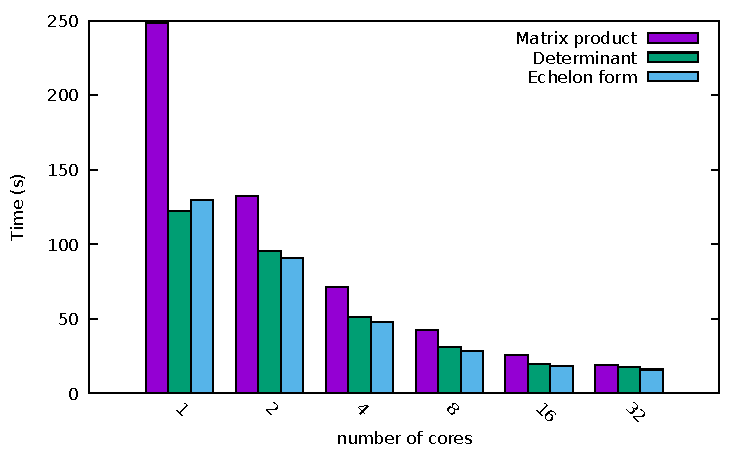
\includegraphics[width=.8\textwidth]{Pictures/histo_bigfoot3}
    \caption{Parallel computation time for some finite field linear algebra operations in SageMath on a 32 core Intel
      Xeon 6130 Gold. Matrices are $20\,000\times 20\,000$ with full rank over $\mathbb{Z}/1\,048\,573\mathbb{Z}$. }
  \end{center}
\end{figure}
\begin{figure}[htb]
  \begin{center}
    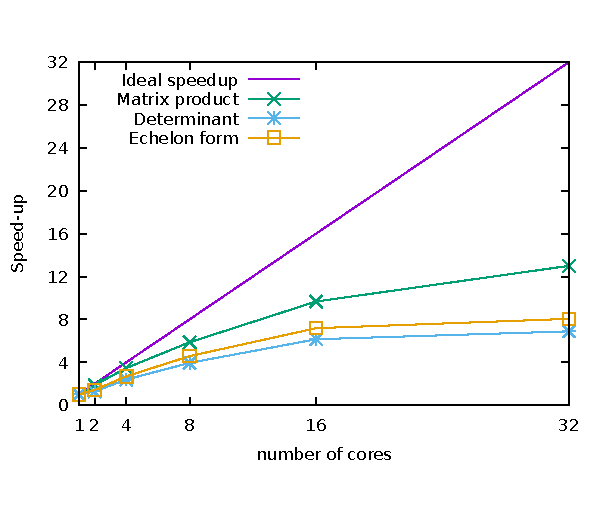
\includegraphics[width=.7\textwidth]{Pictures/speedup_bigfoot3}
    \caption{Parallel speedup for some finite field linear algebra operations in SageMath on a 32 core Intel
      Xeon 6130 Gold. Matrices are $20\,000\times 20\,000$ with full rank over $\mathbb{Z}/1\,048\,573\mathbb{Z}$.}
  \end{center}
\end{figure}

\bibliographystyle{acm}
\bibliography{D3.11}
\end{document}

%%% Local Variables:
%%% mode: latex
%%% TeX-master: t
%%% End:

